\documentclass{svproc}

\usepackage{url}
\usepackage{mdframed}
\usepackage{latexsym}
\usepackage{python}
\usepackage{wrapfig}
\usepackage{epstopdf}
\usepackage{array}
\usepackage{multirow}
\usepackage{caption}
\usepackage{wrapfig}
\usepackage{booktabs}

\usepackage{subfigure}
\usepackage{amssymb}
\usepackage{graphicx}
\usepackage{amssymb}
\usepackage{amsfonts}
\usepackage{bigstrut}

\usepackage[cmex10]{amsmath}
\usepackage{pgfplots}
\usepackage{algorithm}
\usepackage[noend]{algpseudocode}
\usepackage{footmisc}
\captionsetup{compatibility=false}
\usepackage{rotating}
\usepackage{xparse}
\usepackage{todonotes}
\usepackage{comment}
\usepackage{enumitem}
\usepackage{marginnote}
\usepackage{xcolor}
\usepackage{bigstrut}
%\usepackage{paralist}

%\usepackage{tabulary}
\usepackage{colortbl}
\usepackage{cleveref}

\def\UrlFont{\rmfamily}


%
% This one allows us to have a custom DESCRIPTION environment, in which numbers are preceded by a one-letter prefix.
% A short description can be added as an additional parameter to the begin-environment command.
% Successive references will have that very one-letter prefix + number with hyper-reference to it.
%
\RequirePackage{enumitem}
%
\def\requiprefix{T}
%
\newcounter{requicount}
\newlist{requidescr}{description}{1}
\setlist[requidescr,1]{%
	before={\setcounter{requicount}{0}%
		\renewcommand*\therequicount{\arabic{requicount}}},
	,font=\bfseries{\requiprefix}\stepcounter{requicount}\therequicount\normalfont.~\bfseries
}
%
% From https://tex.stackexchange.com/questions/1230/reference-name-of-description-list-item-in-latex
\makeatletter
\def\namedlabel#1{\begingroup
	\def\@currentlabel{\requiprefix\therequicount}%
	\phantomsection\label{#1}\endgroup
}
\makeatother
%
% Usage example:
% \begin{requidescr} % CUSTOM from CDC, with love
%   \item[\namedlabel{req:xaxis} Cluster on Y axis] Something more about that here.
% \end{requidescr}
% I especially like \ref{req:xaxis}.

\begin{document}
\mainmatter
%
%\title{From Time Series to Process Model Forecasting}
\title{Process Model Forecasting Using Time Series Analysis of Event Data}
%
\titlerunning{Process Model Forecasting From Time Series } 
%
\author{Johannes~De~Smedt\inst{1} \and Anton~Yeshchenko\inst{2} \and Artem~Polyvyanyy\inst{3} \and Jochen~De~Weerdt\inst{1} \and Jan~Mendling\inst{2}}
%
\institute{
KU Leuven, Leuven, Belgium\\
\email{\{johannes.desmedt;jochen.deweerdt\}@kuleuven.be}\\
\and
WU Vienna, Vienna, Austria\\
\email{\{anton.yeshchenko;jan.mendling\}@wu.ac.at}
\and
The University of Melbourne, Melbourne, Australia\\
\email{artem.polyvyanyy@unimelb.edu.au}
}
\maketitle

\begin{abstract}
The surge in event data recorded during the execution of business processes is ever-growing and has spurred an array of data-driven process analytics to support and improve how the business processes are performed.
A major strand of such analytics encompasses forecasting how the business processes will unfold into the future, mainly focusing on the next-step, remaining time, and goal-oriented predictions.
The granularity of such approaches lies with the individual events in the process.
In contrast, this work approaches process forecasting at a larger scale and proposes a technique to forecast the entire process model from the available historical event data.
A forecasted model summarizes the anticipated business processes and can be used by process analysts to prepare for the upcoming global and longer-term changes, such as impending process drifts or emerging performance bottlenecks.
To this purpose, event data is reshaped into multiple time series, each representing an evolution of a behavioural aspect of the process model, and collectively specifying the historical evolution of the model.
We then perform time series forecasting to extrapolate the individual series and, concomitantly, the entire model into the future.
Experiments confirm that this approach is capable of informing process analysts about the future evolution of the business processes.
\keywords{Process model forecasting, predictive process modelling, process mining, time series analysis}
\end{abstract}
%
\section{Introduction}\label{sec:introduction}
\section{Related work and motivation}\label{sec:2:motivation}
Within the field of process mining, research on and use of predictive modelling techniques has attracted plenty of attention in the last five years. PPM techniques are usually developed with a specific purpose in mind, ranging from next activity prediction~\cite{evermann2017predicting,DBLP:conf/caise/TaxVRD17}, over remaining time prediction~\cite{verenich2019survey}, to outcome prediction~\cite{kratsch2020machine}. For a systematic literature review of the field, we refer to~\cite{neu2021systematic}. 
Beyond the PPM field, this work is related to previous research on stage-based process mining~\cite{nguyen2016business}, in which a technique is presented to decompose an event log into stages, and work on the detection of time granularity in event logs ~\cite{pourbafrani2020}. 
%Nonetheless, in this work, we employ a more straightforward aggregation, either equitemporal or equisized (cfr. Section~\ref{sec:3a:preliminaries}). 
%\todo[inline]{I find the "nonetheless" sentence confusing. I apparently connects to a point the Pourbafrani paper that is not discussed. And I think also this detailed point should not be discussed here. So the "nonetheless" sentences should be dropped imho. \\Also, I do not understand why Pourbafrani is the only author singled out to be named. Is this paper so striking important? Imho not. So just speak of the paper, not of the author like for all the other papers.}

The shift from fine-granular PPM techniques, including next activity, remaining time, and outcome prediction, to model-based prediction, allows to obtain new insights into the global development of the process.
Consider the example in Figure~\ref{fig:dfg_example_intro} where the road fine traffic management event log\footnote{\url{https://doi.org/10.4121/uuid:270fd440-1057-4fb9-89a9-b699b47990f5}} is partitioned into 100 intervals in which an equal number of DF relations occur.
\begin{figure}
    \centering
    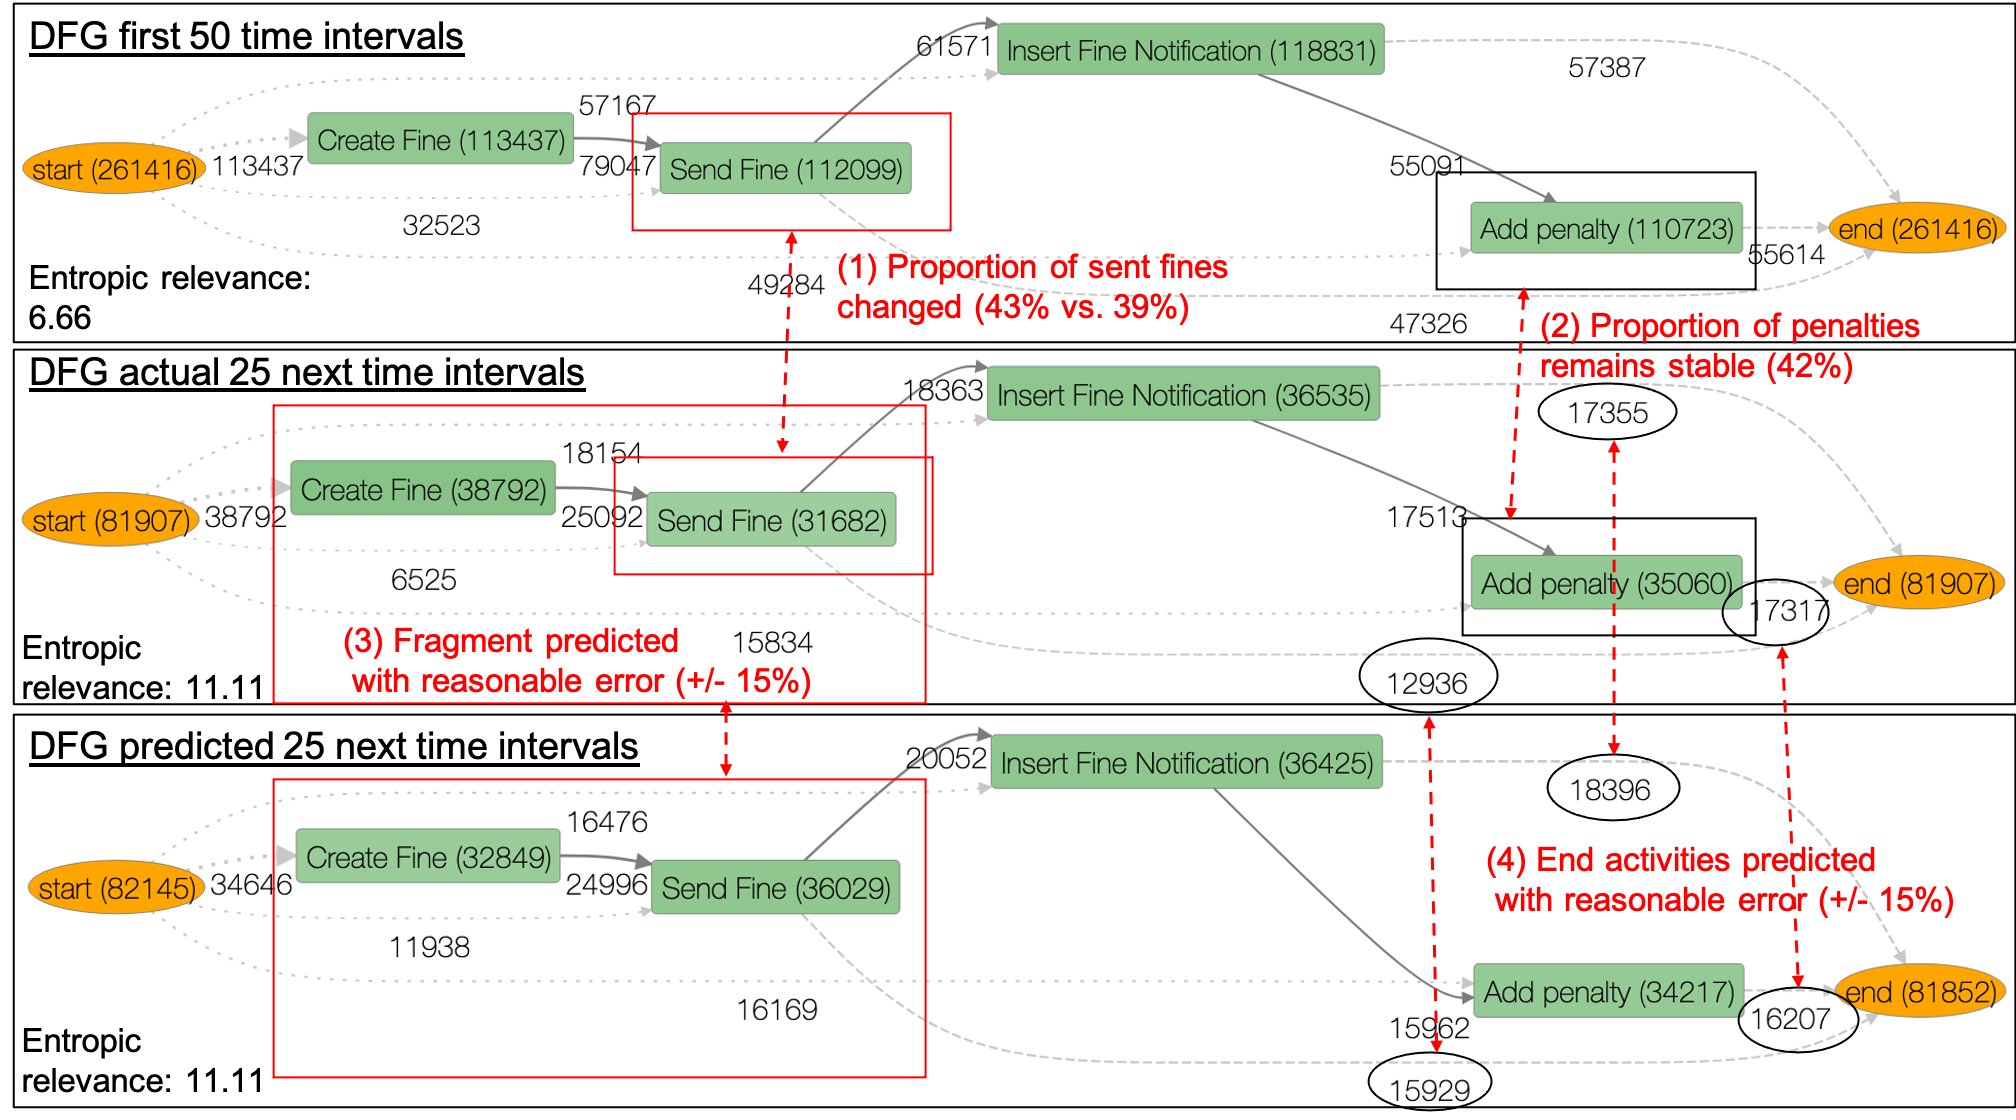
\includegraphics[width=\textwidth]{img/MotExample.png}
    \caption{Directly-follows graphs of the 50 first intervals of the event log, as well as a forecasted and actual DFG of the 25 next intervals.}
    \label{fig:dfg_example_intro}
\end{figure}
The DFs in the first 50 intervals are used to predict the next 25 intervals.
The DFGs show how process model forecasting and change exploration can provide multiple unique insights at a glance:
\begin{enumerate}
    \item Compared to the initial 50 intervals the proportion of fines sent decreases in the later intervals;
    \item The proportion of penalties added remains comparable between the first 50 and next 25 time intervals;
    \item The number of occurrences and arc weights between \emph{Create Fine} and \emph{Send Fine} are predicted with reasonable error (+\-15\%);
    \item The arc weights of the ending activities are predicted with reasonable error (+\-15\%).
\end{enumerate}
These provide insight both in terms of the past and present model ((1)-(2)) and the quality of forecasts between the actual and forecasted model ((3)-(4)).
Being able to construct such forecasts allows stakeholders to make estimates regarding how the overall fine system will evolve and allows to answer questions such as ``How many more fines will be received?'', ``Will the backlog of fines be reduced?'', ``Will all fines be paid'', and `Will the ratio of unpaid fines stay the same?'
This motivating example shows that, where process mining focuses on learning the as-is model to reason about trajectories of future cases and suggest potential repairs and improvements, process model forecasting allows to grasp the future stage of the overall process model in terms of a will-be model. % outcomes of the current as-is process, which allows to shortcut potentially wrong outcomes. 
%\todo[inline]{I found this shortcut-wrong statement hand wavy and misleading. I deleted it.}

A suitable means to evaluate the forecasts quantitatively is entropic relevance \cite{DBLP:conf/icpm/PolyvyanyyMG20}. This measure captures the quality of the discovered and forecasted DFGs with respect to the event logs they represent. 
Entropic relevance penalises the discrepancies in the relative frequencies of traces recorded in the log and described by the DFG as it stands for the average number of bits used to encode a log trace using the DFG, with small values being preferable to large ones.
If the entropic relevance of the forecasted DFG and the actual future DFG with respect to the test log is the same, it suggests that both DFGs represent the future behaviour similarly well. 
The entropic relevance of the historical DFG derived from the training log with respect to the testing log is 6.66 as indicated in Figure \ref{fig:dfg_example_intro}, 
%\todo[inline]{you refer to Fig 1 here, right? Please make that explicit.}
suggesting that the future behaviour shifts and the historical DFG still represents the behaviour in the log better than both the actual and forecasted DFGs which sit at an entropic relevance of 11.11. 

Measurement values are not enough to fully reveal the change of behaviour to the analyst. To this end, we complement the model-level prediction technique with a visualisation system to enable analysts to understand the forthcoming changes to the processes. Various process analysis tasks benefit from process forecasting~\cite{DBLP:conf/bpm/PollPRRR18}, most notably process forecasting helps understanding the incremental changes and adaptations that happen to the process model and to project them into the future. In terms of visualisation principles, we follow the ``Visual Information-Seeking Mantra":~\emph{overview first, zoom and filter, then details-on-demand}~\cite{DBLP:conf/vl/Shneiderman96}. 
%(maybe talk about tasks? not requirements)
Thus, we expect the design of our visualisation system to assist in the following tasks:

\begin{requidescr}
	\item[Identify process adaptations:\namedlabel{req:adaptation}] The visualisation system should assist the user in identifying the changes that happen in the process model of the future in respect to the past;
	\item[Allow for interactive exploration:\namedlabel{req:interactive}] The user should be able to follow the visual information-seeking principles, including overview first, filtering, zooming, and details-on-demand.
\end{requidescr} % CUSTOM from CDC, with love :)

Forecasting entire process models provides a new perspective on predictive process monitoring. 
%Observe that our process model forecasting technique intrinsically puts forwards an entirely new perspective on predictive process monitoring. 
The prediction horizon is substantially longer as compared to what existing next-activity prediction models can achieve. Moreover, where next activity and related PPM techniques have a strong case-level focus, a prediction at the model level provides a more comprehensive picture of the future development of the process.

%\todo[inline]{What comes now as "please..." is unspecific speculation. I tried to eliminate references to our technique in Section 2 altogether. Our technique must be in Section 3. Section 2 is for requirements and other works. However, "please..." goes even further beyond what we actually do. So best simply delete it. It just confuses the reader.}
%Please note that process model forecasting could partially assume goal-oriented prediction, as the forecast DFG allows to answer multiple oftentimes used goal statements pertaining to the execution of a particular activity, or a precedence relationship of a particular activity pair \cite{DBLP:journals/tkdd/TeinemaaDRM19} at the same time. However, our technique is not intended to ``replace'' existing techniques, but rather posits a new yet complementary perspective on PPM.

%Note that the horizon is longer compared with next-step prediction, and that these results would only be obtainable if long next-step predictions were performed.
%Hence, both are complementary by their being used as varying horizons to obtain a full picture of the future development of a process (model).
%Process model forecasting remains complementary with remaining time prediction as well, which could indicate what activities lead to what remaining time.
%The process model forecast can partially assume goal-oriented prediction, as the forecast DFG allows to answer multiple oftentimes used goal statements pertaining to the execution of a particular activity, or a precedence relationship of a particular activity pair \cite{DBLP:journals/tkdd/TeinemaaDRM19} at the same time.

\section{Process model forecasting}\label{sec:methodology}
This section outlines how directly-follows time series are extracted from event logs as well as how they are used to obtain process model forecasts with a range of widely-used forecasting techniques.
Finally, the visualisation of such predictions is introduced.

\subsection{From event log to directly-follows time series}\label{sec:3a:preliminaries}

An event log $L$ which contains the recording of traces $\sigma \in L$ produced by an information system during its execution and contains a sequence of events.
Events in these traces are part of the power set over the alphabet of activities $\Sigma$ which exist in the information system $\sigma=\langle e_1,...,e_{|\sigma|}\rangle \subseteq \Sigma^*$.
Directly follows relations between activities in an event log can be expressed as a counting function over activity pairs $>_L: \Sigma\times\Sigma \to \mathbb{N}$ with $>_L(a_1,a_2) = |\{e_n=a_1,e_{n+1}=a_2, \,\forall e_i\in L\}|$.
Directly follows relations can be calculated on traces and subtraces in a similar fashion.
A Directly Follows Graph (DFG) of the process then exists as the weighted directed graph with the activities as nodes and their DF relations as weights $DFG=(\Sigma,>_L)$.

In order to obtain predictions regarding the evolution of the DFG we construct DFGs for subsets of the log.
Many aggregations and bucketing techniques exist for next-step and goal-oriented outcome prediction \cite{DBLP:conf/caise/TaxVRD17,DBLP:journals/tkdd/TeinemaaDRM19}, e.g., predictions at a point in the process rely on prefixes of a certain length, or particular state aggregations \cite{DBLP:journals/sosym/AalstRVDKG10}.
In the proposed forecasting approach, however, time series instead of cross-sectional data will be used.
Hence, the evolution of the DFGs has to be monitored over intervals of the log where multiple aggregations are possible:
\begin{itemize}
	\item \textbf{Equitemporal aggregation:} each sublog $L_s\in L$ contains a part of the event log of equal time duration. This can lead to sparsely populated sublogs when the events' occurrences are not uniformly spread over time, however, it is easy to apply (on new traces).
	\item \textbf{Equisized aggregation:} each sublog $L_s\in L$ contains a part of the event log where an equal amount of DFs occurred which leads to well-populated sublogs when enough events are available.
\end{itemize}
Tables \ref{tab:eventlog} and \ref{tab:aggregation} provide an example of both.
These aggregations can be useful for the following reasons.
Firstly, equisized aggregation will have a higher likelihood of the underlying DFs approaching a white noise time series which is required for a wide range of time series techniques \cite{hyndman2018forecasting}. 
Secondly, both offer a different threshold at which the forecasting can be applied in practice.
In the case of equisized aggregation, it is easier to quickly construct a desired number of intervals by simply dividing an event log to obtain equisized intervals.
However, most time series techniques rely on the time intervals being of equal size which is embodied by the equitemporal aggregation \cite{kil1997optimum}.
Time series for the DFs $>_{T_{a_1,a_2}}=\langle >_{L_1}(a_1,a_2),\dots,>_{L_s}(a_1,a_2)\rangle, \forall a_1,a_2\in \Sigma\times\Sigma$ can be obtained for all activity pairs where $\bigcup^{L_s}_{L_1}=L$ by applying the aforementioned aggregations to obtain the sublogs.
\begin{table}[htbp]
   \begin{minipage}{.5\textwidth}
   	\centering
    \begin{tabular}{|l|l|l|}
    \toprule
    {Case ID} & Activity &Timestamp \\
    \midrule
    1     & A1    & 11:30 \\
    1     & A2    & 11:45 \\
    1     & A1    & 12:10 \\
    1     & A2    & 12:15 \\
    \midrule
    2     & A1    & 11:40 \\
    2     & A1    & 11:55 \\
    \midrule
    3     & A1    & 12:20 \\
    3     & A2    & 12:40 \\
    3     & A2    & 12:45 \\
    \bottomrule
    \end{tabular}
    \caption{Example event log with 3 traces and 2 activities.}
\label{tab:eventlog}
\end{minipage}
  \begin{minipage}{.5\textwidth}
  	\centering
    \begin{tabular}{|l|c|c|}
    \toprule
    DF    & Equitemporal  & Equisized \\
    \midrule
    $<_{Ls}(A1,A1)$ & (0,1,0) & (1,0,0) \\
    $<_{Ls}(A1,A2)$ & (1,1,1) & (1,1,1) \\
    $<_{Ls}(A2,A1)$ & (0,1,0) & (0,1,0) \\
    $<_{Ls}(A2,A2)$ & (0,0,1) & (0,0,1) \\
    \bottomrule
    \end{tabular}
  \caption{An example of using an interval of 3 used for equitemporal aggregation (75 minutes in 3 intervals of 25 minutes) and equisized intervals of size 2 (6 DFs over 3 intervals)).}
  \label{tab:aggregation}
 \end{minipage}%
\end{table}%

\subsection{From DF time series to process model forecasts}\label{sec:3b:df}

The goal of process model forecasting is to obtain a prediction for future DFGs by combining the predictions of all the DF pairs time series.
To this purpose, we propose to use time series techniques to forecast $\widehat{DFG}_{T+h}=(\Sigma,\{\hat{>}_{T+h|T_{a_1,a_2}}|a_1,a_2\in \Sigma\times\Sigma\})$ for which various algorithms can be used.
In time series modelling, the main objective is to obtain a forecast or prediction $\hat{y}_{T+h|T}$ for a horizon $h\in \mathbb{N}$ based on previous $T$ values in the series $(y_1,...,y_T)$ \cite{hyndman2018forecasting}.
For example, the naive forecast simply uses the last value of the time series $T$ as its prediction $\hat{y}_{T+h|T}=y_T$.
An alternative naive forecast uses the average value of the time series $T$ as its prediction $\hat{y}_{T+h|T}=\frac{1}{T}\Sigma_i^{T} y_i$.

A trade-off exists between approaching DFGs as a multivariate collection of DF time series, or treating each DF separately.
Traditional tme series techniques all use univariate data in contrast with multivariate approaches such as Vector AutoRegression (VAR) models, and machine learning-based methods such as neural networks or random forest regressors.
Despite their simple setup, it is debated whether traditional statistical approaches are necessarily outperformed by machine learning methods. 
\cite{makridakis2018statistical} found that this is not the case on a large number of datasets and note that the machine learning algorithms require significantly more computational power, a result that was later reaffirmed although it is noted that hybrid solutions are effective \cite{makridakis2020m4}.
Especially for longer horizons, traditional time series approaches still outperform machine learning-based models.
Given the potentially high number of DF pairs in a process' DFG, the proposed approach uses a time series algorithm for each DF series separately.
VAR models would require a high number of intervals (at least as many as there are DFs times the lag coefficient) to be able to estimate all parameters of such a high number of time series despite their potentially strong performance \cite{thomakos2004naive}.
Machine learning models could potentially leverage interrelations between the different DFs but again would require long training times to account for dimensionality issues due to the potentially high number of DFs. 
Therefore, in this paper, traditional time series approaches are chosen and applied to the univariate DF time series where these have at least 1 observation per sublog/time interval present.

We briefly discuss smoothing models, autoregressive, moving averages and ARIMA models, and varying variance models which make up the main families of traditional time series forecasting \cite{hyndman2018forecasting}.
A wide array of such forecasting techniques exist, ranging from simple models such as naive forecasts over to more advanced approaches such as exponential smoothing and auto-regressive models.
Many also exist in a seasonal variant due to their application in contexts such as sales forecasting.

A Simple Exponential Smoothing (SES) model uses a weighted average of past values where their importance exponentially decays as they are further into the past where Holt's models introduce a trend in the forecast, meaning the forecast is not flat.
Exponential smoothing models often perform very well despite their simple setup \cite{makridakis2018statistical}.
AutoRegressive Integrating Moving Average (ARIMA) models are based on auto-correlations within time series. 
They combine auto-regressions with a moving average over error terms.
It is established by a combination of an AutoRegressive (AR) model of order $p$ uses the past $p$ values in the time series and applies a regression over them and a Moving Average (MA) model of order $q$ which creates a moving average of the past forecast errors.
Given the necessity of using a white noise series for AR and MA models, data is often differenced to obtain such series.
ARIMA models then combine both AR and MA models where the integration is taking place after modelling as these models are fitted over differenced time series.
ARIMA models are considered to be one of the strongest time series modelling techniques.
An extension to ARIMA which is widely used in econometrics exists in (Generalized) AutoRegressive Conditional Heteroskedasticity ((G)ARCH) models \cite{francq2019garch}.
They resolve the assumption that the variance of the error term has to be equal over time, but rather model this variance as a function of the previous error term.
For AR-models, this leads to the use of ARCH-models, while for ARMA models GARCH-models are used as follows.
An ARCH(q) model captures the change in variance by allowing it to both gradually increase over time, or to allow for short bursts of increased variance.
A GARCH(p,q) model combines both the past values of observations as well as the past values of variance.
(G)ARCH models often outperform ARIMA models in contexts such as the prediction of financial indicators of which the variance often changes over time \cite{francq2019garch}.









\subsection{Process change exploration}\label{sec:3c:pce}


% as has been shown the prediction is nice but it is difficult to derive the insignts 
% definition of the visualization
% humans cannot comprehend the results and we need visualzation 
% (new functions on vis that ar enot mentioned before should be mentioned?)

%%%
% outline:
% 0. short intro
% 1. user tasks
% 2. design (and what supports design)
% 3. implementation and the resources.
%%%

In~\Cref{sec:3a:preliminaries} we described the approach for forecasting process models. To that end, gaining actual insights from such predicted values remains a difficult task for the analyst. This section sets off to present the design of a novel visualisation system to aid analysts in the exploration of the event logs and their corresponding (forecasted) discovered process models.

Following the user tasks~\ref{req:adaptation} and~\ref{req:interactive}, we designed a Process Change Exploration (PCE) system to support the interpretation of the process model forecasts. PCE is an interactive visualisation system that consists of three connected views.


%In order to design the system we first established user tasks as a basis for the system design decisions. 


%To derive the user tasks we focus on the requirements of process mining analysis with respect to process forecasting and visualization principles. The authors of~\cite{DBLP:conf/bpm/PollPRRR18} discuss the opportunities for process forecasting. They describe that the utility of process forecasting is an understanding of the incremental changes or adaptations that happen to the process model into the future. In designing an explorative visualization system, we also followed the "Visual Information-Seeking Mantra:"~\emph{overview first, zoom and filter, then details-on-demand}~\cite{DBLP:conf/vl/Shneiderman96}. 
%%(maybe talk about tasks? not requirements)
%Thus, we expect the design of our system to assist in the following tasks:
%
%%requirements for the visualization based on the related literature and experience working with event sequence data. 
%
%\begin{requidescr}
%	\item[Identify process adaptations:\namedlabel{req:adaptation}] The visualization system should assist the user in identifying the changes that happen in the process model of the future in respect to the past;
%	\item[Allow for interactive exploration:\namedlabel{req:interactive}] The user should be able to follow the visual information-seeking principles, including overview first, filtering, zooming, details-on-demand principles.;
%\end{requidescr} % CUSTOM from CDC, with love :)




\textbf{Adaptation Directly-Follows Graph (aDFG) view.} This is the main view of the visualisation that will show the model of the process. In order to accomplish the task~\ref{req:adaptation}, we modify the DFG syntax. In order to display the process model adaptation from time range $T_{i_0,j_0}, i_0<j_0$ to $T_{i_1,j_1}, i_1<j_1$ we display the union of the process models of these regions, annotating the places and transitions with the numbers of both ranges. We colour the aDFG as follows: we use colour saturation to show the places with higher values. We colour transitions with a diverging saturation (red-black-green) schema. This colouring applies red colour to transitions that are dominant in the $T_{i_0,j_0}$ range, and green if transitions are dominant in the $T_{i_1,j_1}$ range, otherwise the transition is close to black. For coloring transitions, we used idea of the three colour schema from~\cite{DBLP:conf/grapp/KriglsteinR12}.

\textbf{Timeline view with brushed regions.} This view represents the area chart graph that shows how the number of activity executions change with time. The area chart colour is split in two parts, one for the actual data, and the other one to show the time range where values are predicted. Analyst can brush one region in order to zoom in, creating one region of interest $T_{i_0,j_0}, i_0<j_0$ that is displayed on the DFG. Analyst can also brush two regions of the area chart to select two time ranges, updating the DFG to aDFG representation. The brushed regions are coloured accordingly to the schema for colouring aDFG transitions. The earlier brushed region is coloured in the red, while the second one is coloured green. 

\textbf{Activity and path sliders.} We adopt two sliders that are used to simplify the DFG~\cite{leemans2019directly} and the aDFG for detailed exploration of the models.

Based on the described views, we conjecture that the analyst is able to accomplish the tasks~\ref{req:adaptation}, and~\ref{req:interactive} with ease.



%The interactive system consists of three parts. Part b shows the timeline of the data (green region), and forecasted values (grey region). The user can brush one or two regions (in this b.1 and b.2) on this graph to see the filtered for that time range process model or a difference between two process models. The main view (a) represents the directly follows change graph that shows the difference between two brushed regions. The c.1 and c.2 are the usual filters on the number of paths and activities to aid simplification the visual representation




%\begin{figure}
%	\centering
%	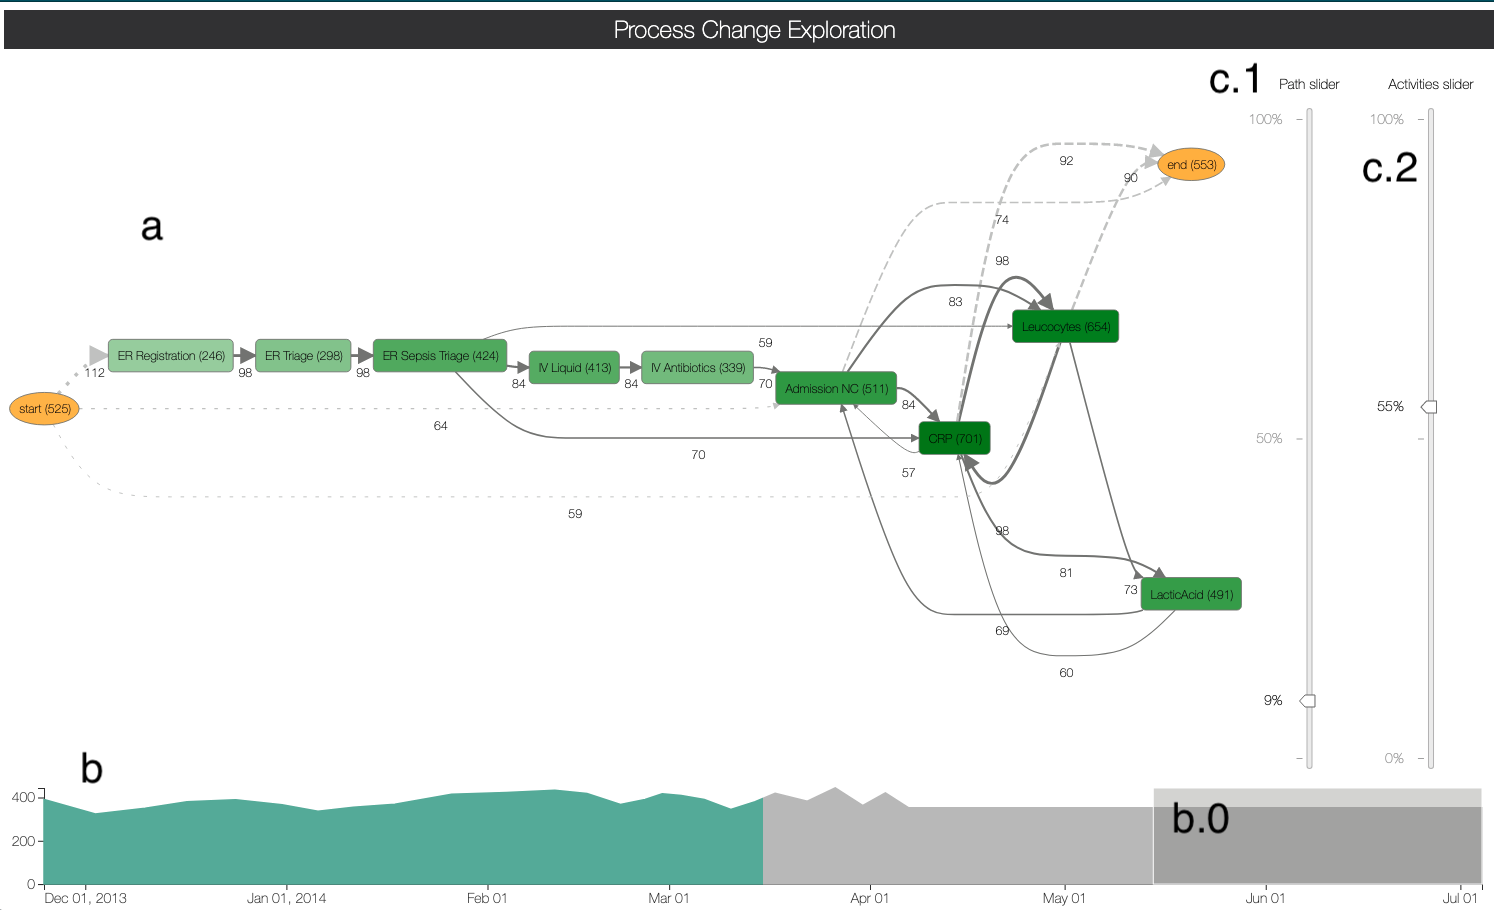
\includegraphics[width=\textwidth]{img/vis/vis-system-one-brush.png}
%	\caption{Process Change Exploration (PCE) system.} 
%	\label{fig:vis-one-brushes}
%\end{figure}

%Process Change Exploration (PCE) system. The interactive system consists of three parts. Part b shows the timeline of the data (green region), and forecasted values (grey region). The user can brush one time range (in this b.0) on this graph to see the filtered for that time range process model. The main view (a) represents the directly follows graph of that region. The c.1 and c.2 are the usual filters on the number of paths and activities to aid simplification the visual representation}

%
%\noindent\textbf{%
%Implementation. 
%} 


%\noindent\textbf{%
%	User interface
%} The Figure~\ref{fig:vis-two-brushes} displays the screenshot of the PCE visualization system. 
%We improve upon the notion of Directly-Follows graph~\cite{leemans2019directly} that is widely used in process mining research and practice. We use the ideas from the version graph~\cite{DBLP:conf/grapp/KriglsteinR12} on how to represent the change between versions of the graph with coloring of the transitions. 



% as has been shown the prediction is nice but it is difficult to derive the insignts 
% definition of the visualization
% humans cannot comprehend the results and we need visualzation 
% (new functions on vis that ar enot mentioned before should be mentioned?)

%%%
% outline:
% 0. short intro
% 1. user tasks
% 2. design (and what supports design)
% 3. implementation and the resources.
%%%



\section{Implementation and evaluation}\label{sec:experiment}
In this section, an experimental evaluation over three real-life event logs is reported.
The aim of the evaluation is to measure to what extent the forecasted process models/DFGs are capable of correctly reproducing actual future DFGs in terms of their arc weights (measured as deviations or errors), as well as whether they are capable of reproducing the same process model behaviour (measured against the behaviour of the baseline actual DFG).
This is done at various parts of the trace, i.e. forecasts for the middle of the event logs up to the later parts of the event log to capture the robustness of the forecasting techniques in terms of the amount of data required to obtain good prediction results.
This is done for both the equisized and equitemporal aggregation.

\subsection{Re-sampling and test setup}
In order to obtain training data, time series are obtained by specifying a number of intervals (i.e. time steps in the DF time series) using either equitemporal or equisize aggregation a described in Section \ref{sec:preliminaries}.
Time series algorithms are parametric and sensitive to sample size requirements \cite{hanke2001business}.
Depending on the number of parameters a model uses, a minimum size of at least 50 steps is not uncommon, although typically model performance should be monitored at a varying number of steps.
In the experimental evaluation, the event logs are divided into 100 time steps with a varying share of training and test steps:. A constant and long horizon $h=25$ is used meaning all test sets contain 25 intervals, but the training sets are varied from $ts=25$ to $ts=75$ steps, meaning the forecasts progressively target the prediction of steps 25-50 (the second quarter of intervals) over to 75-100 (the last quarter of intervals).
This allows to both inspect the difference in results when only few data points are used, and whether there is a difference forecasting data points in the middle or towards the end of the available event data.

Resampling is applied based on a 10-fold cross-validation constructed following a rolling window approach for all horizon values $h\in[1,25]$ where a recursive strategy is used to iteratively obtain $\hat{y}_{t+h|T_{t+h-1}}$ with $(y_1,\dots,y_{T},\dots,\hat{y}_{t+h-1})$ \cite{weigend2018time}.
10 training sets are hence constructed for each training set length $ts$ and exist from $(y_1,\dots,y_{T-h-f})$ and the test sets from $(y_{T-h-f+1},\dots,y_{T-f})$ with $f\in[0,9]$ the fold index \cite{bergmeir2012use}.
While direct strategies with a separate model for every value of $h$ can be used as well and avoid the accumulation of error, they do not take into account statistical dependencies for subsequent predictions.

Three widely-used event logs are used: the 2012 BPI challenge log\footnote{\url{https://doi.org/10.4121/uuid:3926db30-f712-4394-aebc-75976070e91f}}, the Sepsis cases event log\footnote{\url{https://doi.org/10.4121/uuid:915d2bfb-7e84-49ad-a286-dc35f063a460}}, and the Road Traffic Fine Management Process log (RTFMP) event log (see Section \ref{sec:2:motivation}.
Each of these logs has a diverse set of characteristics in terms of case and activity volume, as well as average trace length as can be seen in Table \ref{tab:eventlogs}.
\begin{table}[htbp]
  \centering
    \begin{tabular}{lrrr}
    \toprule
    \textbf{Event log} & \multicolumn{1}{l}{\textbf{\# cases}} & \multicolumn{1}{l}{\textbf{\# activities}} & \multicolumn{1}{l}{\textbf{Average trace length}} \\
    \midrule
    \textbf{BPI 12} & 13,087 & 36    & 20.020 \\
    \textbf{Sepsis} & 1,050 & 16    & 14.490 \\
    \textbf{RTFMP} & 150,370 & 11    & 3.734 \\
    \bottomrule
    \end{tabular}%
  \caption{Overview of the characteristics of the event logs used in the experimental evaluation.}
  \label{tab:eventlogs}%
\end{table}%

An example of applying the equisize or equitemporal aggregation to the Sepsis event log with 100 intervals results in the DF time series of Figure \ref{fig:sepsists} where the DF occurrences of the most frequently occurring activity pair is included.
For the equisized aggregation the number of DFs is indeed relatively stable over the log's timeline where for the equitemporal aggregation a noticeable decline of DF pairs is visible towards the end of the series.
This phenomenon is typical in event logs, as processes typically have particular endpoint activities, but can also be due to the unequal distribution of events over the event log's time line.
If the level of occurrences of the DF pair is low and close to 0, the series might be too unsuitable for analysis with white noise series analysis techniques that assume stationarity.
Ideally, every time series is tested using a stationarity test such as the Dickey-Fuller unit root test \cite{leybourne1995testing} and an appropriate lag order is established for differencing. 
Furthermore for each algorithm, especially ARIMA-based models, (partial) auto-correlation could establish the ideal $p$ and $q$ parameters.
However, for the sake of simplicity and to avoid solutions where each activity pair has to have different parameters, various values are used for $p$, $d$, and $q$ and applied to all DF pairs where only the best-performing are reported below for comparison with the other time series techniques.
The results contain the best-performing representative of each forecasting family.
\begin{figure}[tb]
	\centering
	\subfigure[Most common DF - equisize]{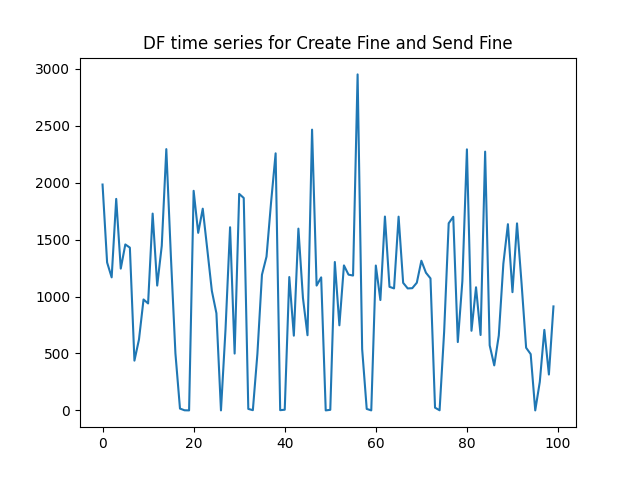
\includegraphics[width=0.39\textwidth]{./img/rtfmp_1.png}}
	\subfigure[Most common DF - equitemp]{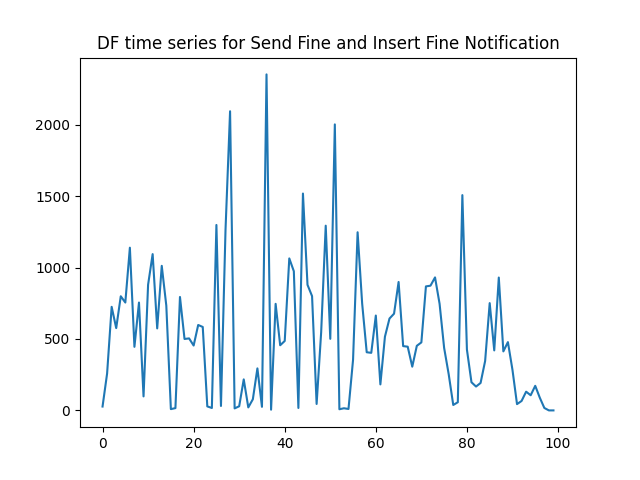
\includegraphics[width=0.39\textwidth]{./img/rtfmp_1_t.png}}
	\caption{RTFMP}
	\label{fig:sepsists}
\end{figure}

\subsection{Evaluation criteria}
Given that we want to evaluate the capability of the approach to accurately predict the evolution of the process model, the combination of all DF predictions to obtain a global DFG prediction is considered.
The following two criteria are used:
\begin{itemize}
	\item \textbf{Cosine distance:} measures the distance between two vectors and is often used to compare graph distance. This metric is used to compare the DFG's edge weight matrices between the actual and predicted number of DF relations.
	\item \textbf{Entropic relevance:} a measure for stochastic conformance checking computed as the average number of bits required to compress each of the log’s traces based on the structure and information about relative likelihoods provided by the model \cite{DBLP:conf/icpm/PolyvyanyyMG20}.
\end{itemize}
These criteria balance a predictive and structural evaluation of the algorithms and report on both the numeric performance common in a forecasting setting as well as their appropriateness in terms of reproducing a structurally usable process model which allows for the observed process behaviour.
In both cases a lower score is better.
The entropic relevance also allows to compare the adequacy the forecasted DFGs with the actual DFGs.

\subsection{Results}
All pre-processing was done in Python with a combination of \emph{pm4py}\footnote{\url{https://pm4py.fit.fraunhofer.de}} and the \emph{statsmodels} package \cite{seabold2010statsmodels}. 
The code and full results are available here\footnote{\url{https://github.com/JohannesDeSmedt/pmf}}.
Figures \ref{fig:rtfmp_equisize} and \ref{fig:rtfmp_equitemp} contain visualisations of the cosine distance and entropic relevance for the RTFMP log, and Table \ref{tab:result_table} contains the mean absolute percentage error (MAPE) of the actual and forecasted DFGs in terms of entropic relevance.
\begin{table}[htbp]
  \centering
  \resizebox{0.65\textwidth}{!}{
    \begin{tabular}{|c|l|ccc|ccc|ccc|}
\cmidrule{3-11}    \multicolumn{1}{r}{} &       & \multicolumn{3}{c|}{\textbf{BPI 12}} & \multicolumn{3}{c|}{\textbf{Sepsis}} & \multicolumn{3}{c|}{\textbf{RTFMP}} \\
    \multicolumn{1}{r}{} &       & \textbf{50} & \textbf{75} & \textbf{100} & \textbf{50} & \textbf{75} & \textbf{100} & \textbf{50} & \textbf{75} & \textbf{100} \\
    \midrule
    \multirow{5}[2]{*}{\begin{sideways}\textbf{equisize}\end{sideways}} & \textbf{nav} & \textbf{2.63} & 2.55  & 2.23  & 8.66  & 7.19  & 5.85  & \textbf{35.10} & \textbf{19.63} & 17.03 \\
          & \textbf{arima212} & 4.49  & \textbf{2.31} & \textbf{2.20} & NA    & 8.93  & 6.55  & 40.65 & NA    & 20.71 \\
          & \textbf{ar2} & 2.91  & 2.69  & 2.22  & 10.45 & 6.49  & 5.14  & NA    & NA    & \textbf{14.44} \\
          & \textbf{hw} & 2.71  & 2.41  & 2.22  & 8.25  & 7.52  & 6.20  & 43.06 & 24.09 & 20.20 \\
          & \textbf{garch} & 3.02  & 3.02  & 2.26  & \textbf{7.66} & \textbf{6.14} & \textbf{4.95} & 37.65 & 22.93 & 15.12 \\
    \midrule
    \multicolumn{1}{|c|}{\multirow{5}[2]{*}{\begin{sideways}\textbf{equitemp}\end{sideways}}} & \textbf{nav} & 3.75  & \textbf{3.09} & 3.11  & 9.77  & 6.99  & NA    & 20.81 & 12.96 & 15.19 \\
          & \textbf{arima212} & 5.35  & 4.16  & \textbf{2.83} & 14.87 & 7.88  & NA    & 33.03 & 13.79 & \textbf{14.48} \\
          & \textbf{ar2} & NA    & 3.19  & 3.13  & 15.35 & 6.51  & NA    & NA    & 13.06 & 15.38 \\
          & \textbf{hw} & 4.10  & 3.21  & 3.06  & \textbf{7.98} & 6.08  & NA    & 26.15 & 13.29 & 15.77 \\
          & \textbf{garch} & \textbf{3.74} & 3.19  & 3.17  & 23.00 & \textbf{5.68} & NA    & \textbf{19.68} & \textbf{11.68} & 14.64 \\
    \bottomrule
    \end{tabular}%
    }
    \caption{Overview of the mean percentage error in terms of entropic relevance.}
  \label{tab:result_table}%
\end{table}%


The MAPE results show that many techniques are capable of staying well below the 5\% difference for BPI 12 (except for ARIMA after 50 intervals) with the naive forecasting baseline performing competitively with the slightly outperforming ARIMA(2,1,2) model in some cases.
For the Sepsis dataset, results below the 10\% line can be achieved by many techniques, with GARCH performing best for equisize and Holt-Winters for equitemporal aggregation.
Given the few DF occurrences in the later part of the event log, no results can be produced for the equitemporal aggregation.
Finally, the RTFMP only achieves below 15\% MAPE for the 100 intervals or equitemporal aggregation.
Figures \ref{fig:rtfmp_equisize} and \ref{fig:rtfmp_equitemp} show that GARCH indeed performs well in terms of low entropic relevance, but not cosine distance.
Besides, it shows that most techniques perform similarly in terms of entropic relevance.

Overall, there is no clear forecasting technique that stands out over the whole line, while the naive baseline often performs adequately and GARCH reporting best or close-to-best results in at least half the cases.
The errors are higher when fewer intervals are used for training with 100 intervals ($ts=75$) resulting in the lowest MAPE for all three datasets.
Nevertheless, even for 75 intervals ($ts=50$) the results are closer to the 100 than the 50 interval setup.
It also appears that equitemporal aggregation results is lower forecasting errors when the training set is small.

\begin{figure}
    \centering
    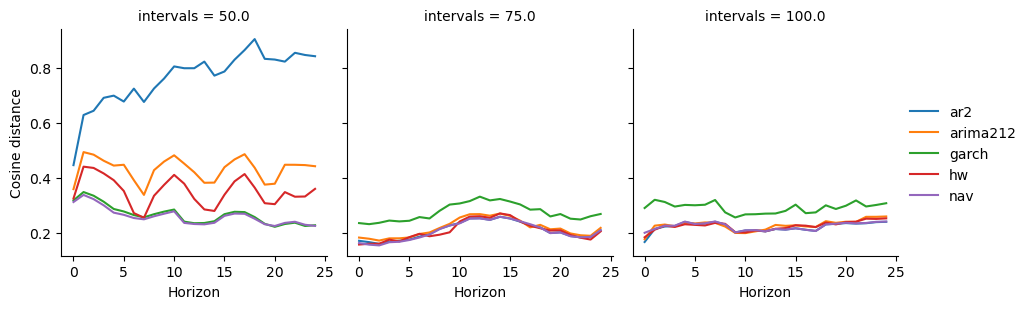
\includegraphics[width=0.8\textwidth]{img/rtfmp_cosine_small_equisize.png}
    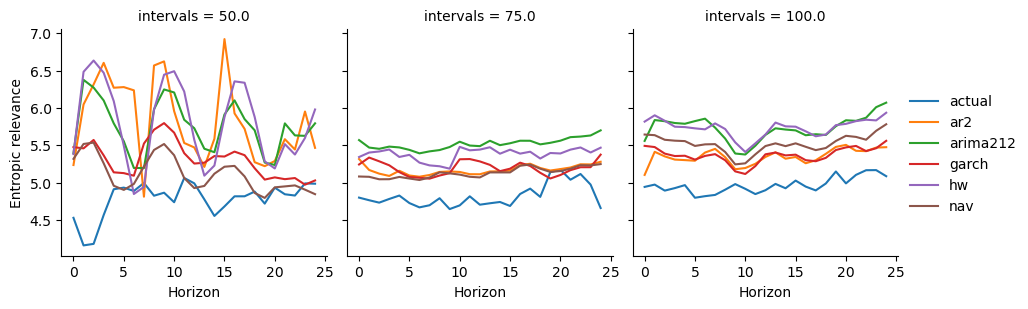
\includegraphics[width=0.8\textwidth]{img/rtfmp_entropic_small_equisize.png}
    \caption{Results for equisize aggregation for the RTFMP event log.}
    \label{fig:rtfmp_equisize}
\end{figure}
\begin{figure}
    \centering
    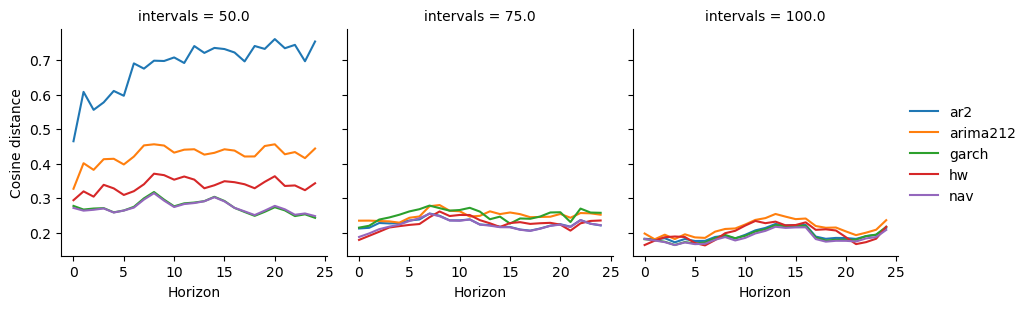
\includegraphics[width=0.8\textwidth]{img/rtfmp_cosine_small_equitemp.png}
    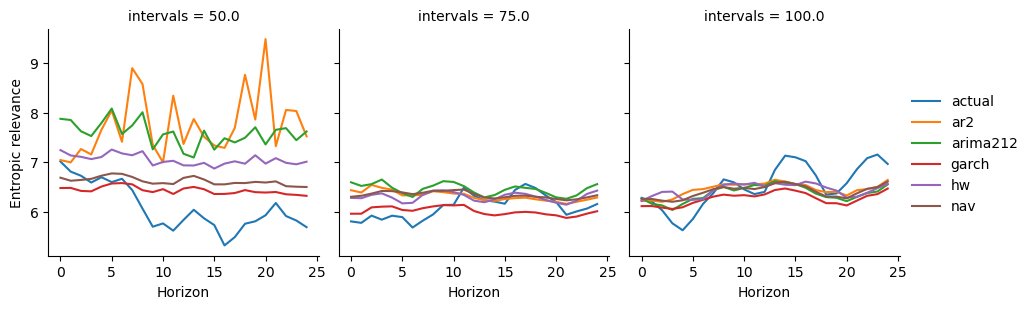
\includegraphics[width=0.8\textwidth]{img/rtfmp_entropic_small_equitemp.png}
    \caption{Results for equitemporal aggregation for the RTFMP event log.}
    \label{fig:rtfmp_equitemp}
\end{figure}

\subsection{Visualising Process Model Forecasts}\label{sec:visualisation}

In~\Cref{sec:experiment} we evaluated forecasting results, ensuring the relevance of the predicted process models. To that end, gaining actual insights from such predicted data remains a difficult task for the analyst. This section sets off to present the implementation of a novel visualization system to aid analysts in exploration of the event logs. The process of designing and implementing the system started by designing several prototypes that undergone rounds of discussions to mature into the implemented visualization system. 

The design of the PCE system is shown in Figure~\ref{fig:vis-two-brushes}. It shows an interactive visualization system with several connected views. The system is implemented with D3.js JavaScript library and is available at~\footnote{\url{google.com}}.


\begin{figure}
	\centering
	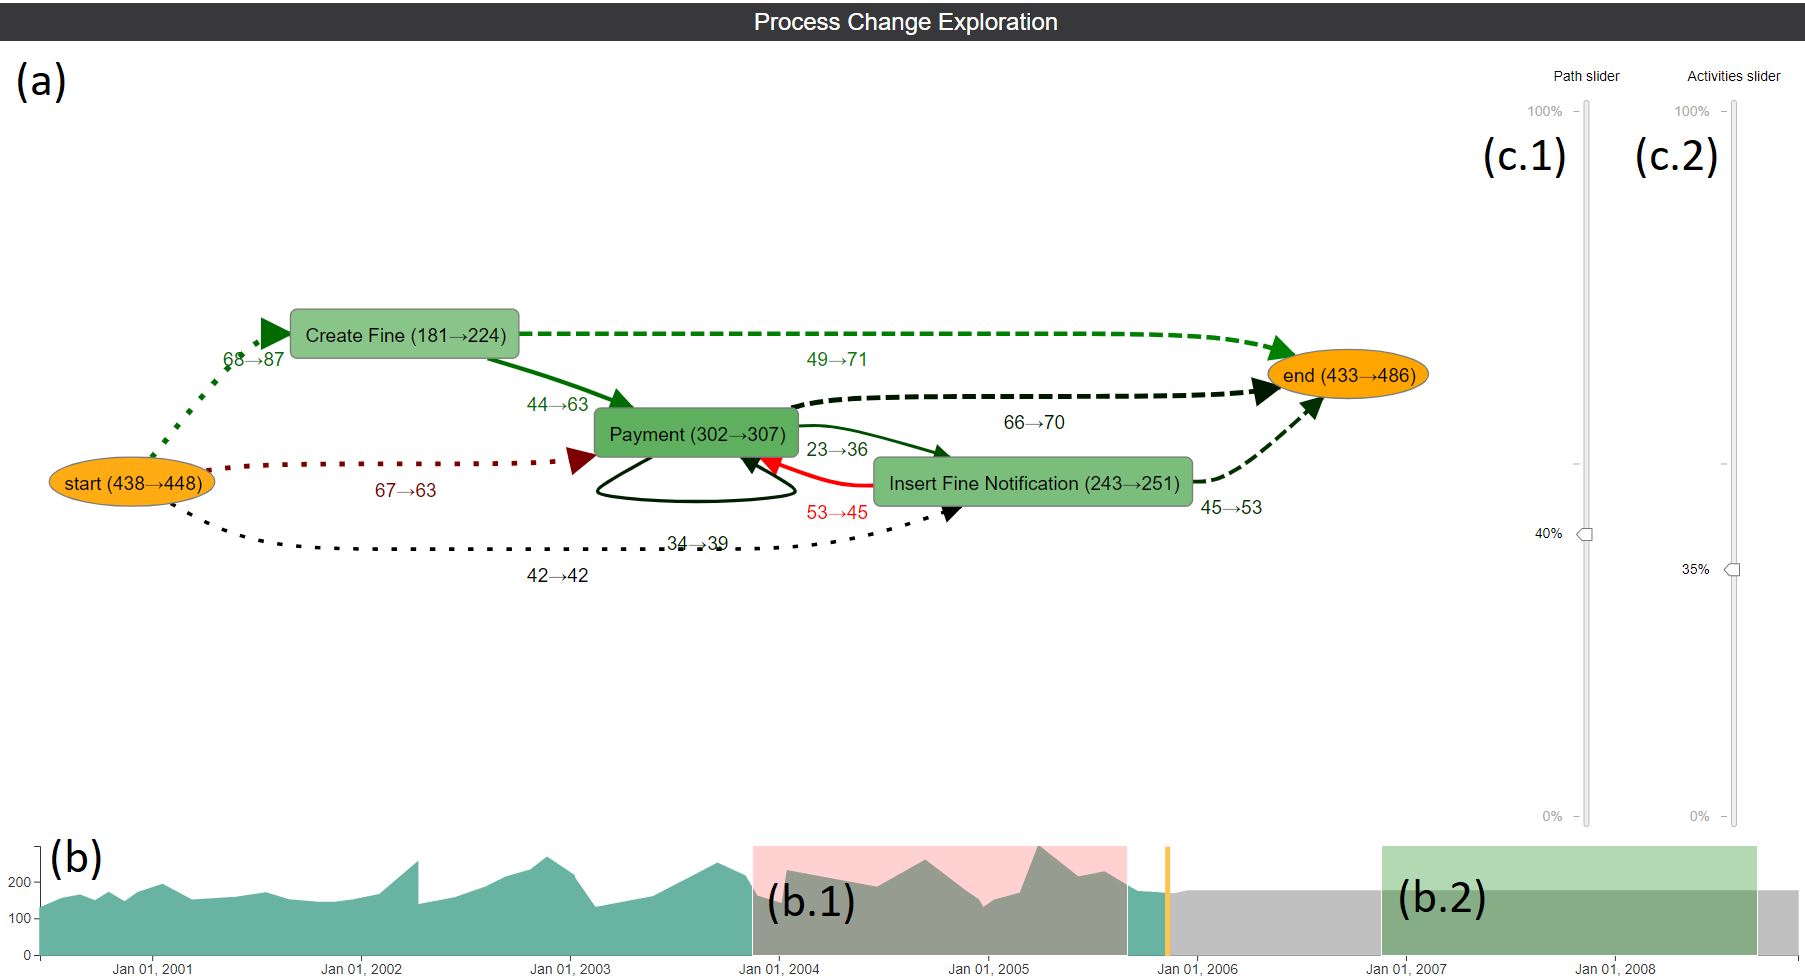
\includegraphics[width=\textwidth]{img/vis/actual-predicted-two-brushed-regions-system.PNG}
	\caption{Process Change Exploration (PCE) system.~\emph{(a)} shows~\emph{Adaptation Directly-Follows Graph (aDFG)} view.~\emph{(b)} shows the \emph{Timeline view with brushed regions} view. Users can brush one or more regions on this graph in order to filter the scope of the analysis~\emph{(b.1}, and~\emph{b.2)}. Two additional views~\emph{(c.1)}, and~\emph{(c.2)} show the \emph{activity and path sliders}.} 
	\label{fig:vis-two-brushes}
\end{figure}
\section{Visualising Process Model Forecasts}\label{sec:visualisation}


% as has been shown the prediction is nice but it is difficult to derive the insignts 
% definition of the visualization
% humans cannot comprehend the results and we need visualzation 
% (new functions on vis that ar enot mentioned before should be mentioned?)

%%%
% outline:
% 0. short intro
% 1. user tasks
% 2. design (and what supports design)
% 3. implementation and the resources.
%%%

In the Section~\ref{sec:experiment} we evaluated forecasting results, ensuring the relevance of the predicted process models. To that end, gaining actual insights from such predicted data remains a difficult task for the analyst. This section sets off to present the design of a novel visualization system to aid analysts in exploration of the event logs.

%The evaluation Section~\ref{sec:experiment} has shown a good performance of the prediction algorithms for the process model forecasts. To that end, deriving insights from such predicted data remains a difficult task for the analyst. In this section we present the design of visualization system that aids analysts in exploration of the past and future of the processes.

We designed a Process Change Exploration (PCE) system to support the interpretation of the process model forecasts. In order to design the system we first established user tasks as a basis for the system design decisions. To derive the user tasks we focus on the requirements of process mining analysis with respect to process forecasting and visualization principles. The authors of~\cite{DBLP:conf/bpm/PollPRRR18} discuss the opportunities for process forecasting. They describe that the utility of process forecasting is an understanding of the incremental changes or adaptations that happen to the process model into the future. In designing an explorative visualization system, we also followed the "Visual Information-Seeking Mantra:"~\emph{overview first, zoom and filter, then details-on-demand}~\cite{DBLP:conf/vl/Shneiderman96}. 
%(maybe talk about tasks? not requirements)
Thus, we expect the design of our system to assist in the following tasks:

%requirements for the visualization based on the related literature and experience working with event sequence data. 

\begin{requidescr}
	\item[Identify process adaptations:\namedlabel{req:adaptation}] The visualization system should assist the user in identifying the changes that happen in the process model of the future in respect to the past;
	\item[Allow for interactive exploration:\namedlabel{req:interactive}] The user should be able to follow the visual information-seeking principles, including overview first, filtering, zooming, details-on-demand principles.;
\end{requidescr} % CUSTOM from CDC, with love :)


\begin{figure}
	\centering
	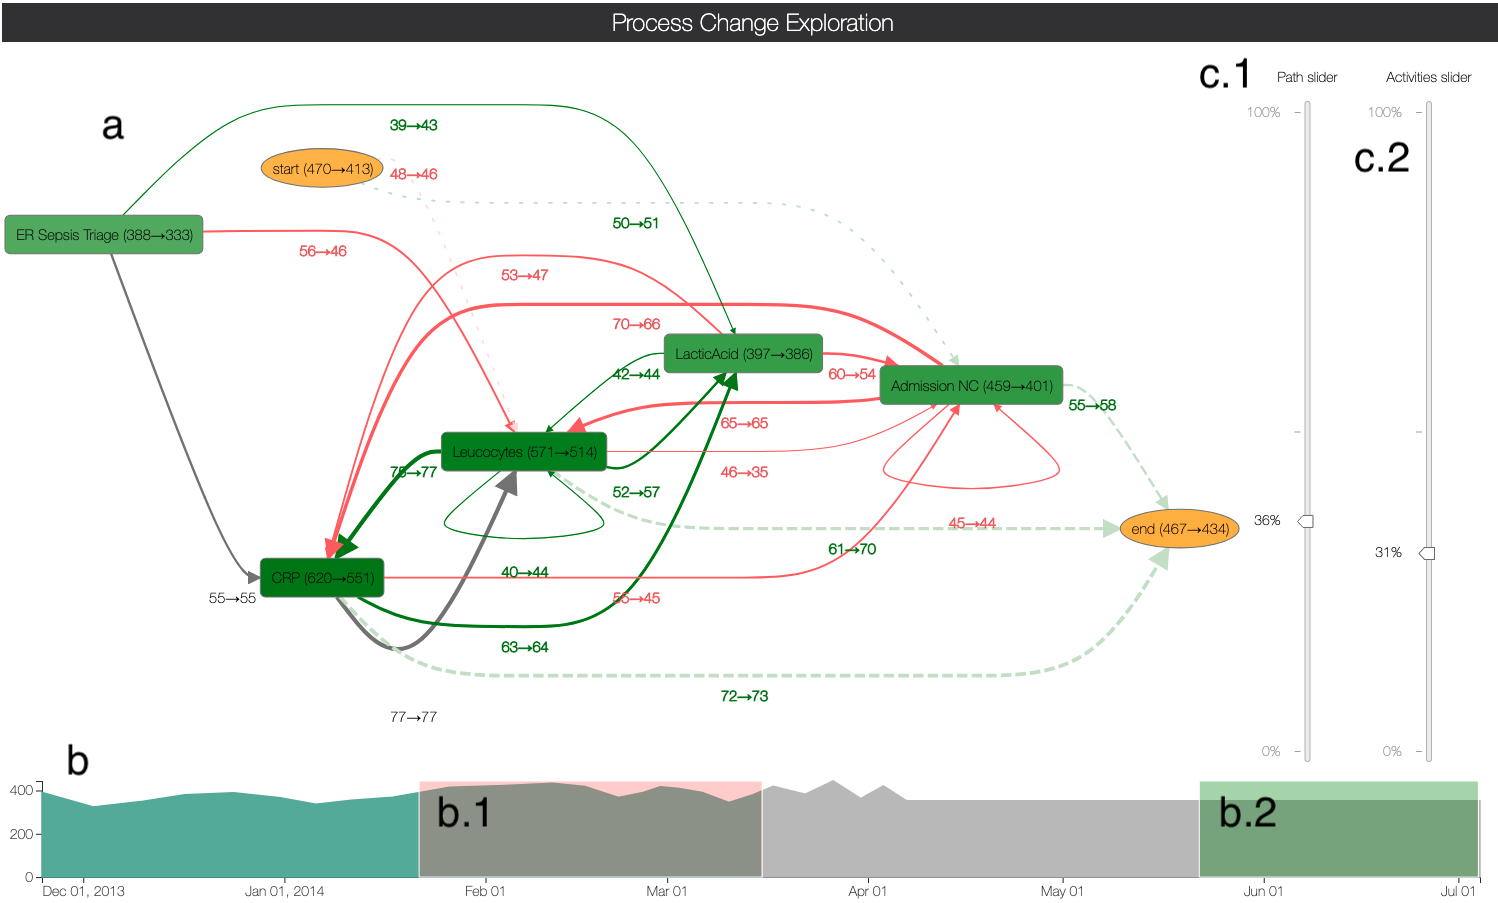
\includegraphics[width=\textwidth]{img/vis/vis-system-two-brushes.png}
	\caption{Process Change Exploration (PCE) system.~\emph{(b)} is the activity timeline view,~\emph{(a)} main Directly-follows graph view,~\emph{(c.1), (c.2)} additional filtering views.} 
	\label{fig:vis-two-brushes}
\end{figure}

%The interactive system consists of three parts. Part b shows the timeline of the data (green region), and forecasted values (grey region). The user can brush one or two regions (in this b.1 and b.2) on this graph to see the filtered for that time range process model or a difference between two process models. The main view (a) represents the directly follows change graph that shows the difference between two brushed regions. The c.1 and c.2 are the usual filters on the number of paths and activities to aid simplification the visual representation


The design of the PCE system is shown in Figure~\ref{fig:vis-two-brushes}. It shows an interactive visualization system with several connected views. The view~\emph{(b)} shows the area graph for the number of activities executed per each period. The green area represents the actual data, and the grey region represents the predicted values. Users can brush one or more regions on this graph in order to filter the scope of the analysis~\emph{(b.1}, and~\emph{b.2)}. If a user brushes two regions then the earlier will be color-coded in red, and the later color-coded in green. The main DFG view~\emph{(a)} is showing the directly follows graph of the brushed region when none or one region is selected or the difference between two brushed regions when two regions are brushed. In case the difference is showed, the red transitions are used to show the decrease in executions, green to show the increase and grey in case of stable behavior. For coloring, we used ideas from~\cite{DBLP:conf/grapp/KriglsteinR12}. Two additional views~\emph{(c.1)}, and~\emph{(c.2)} allow for the standard filtering~\cite{leemans2019directly} of activities and paths.

The process of designing and implementing the system started by designing several prototypes that undergone rounds of discussions to mature into the implemented visualization system. The system is implemented with D3.js JavaScript library and is available at~\footnote{\url{google.com}}.

%\begin{figure}
%	\centering
%	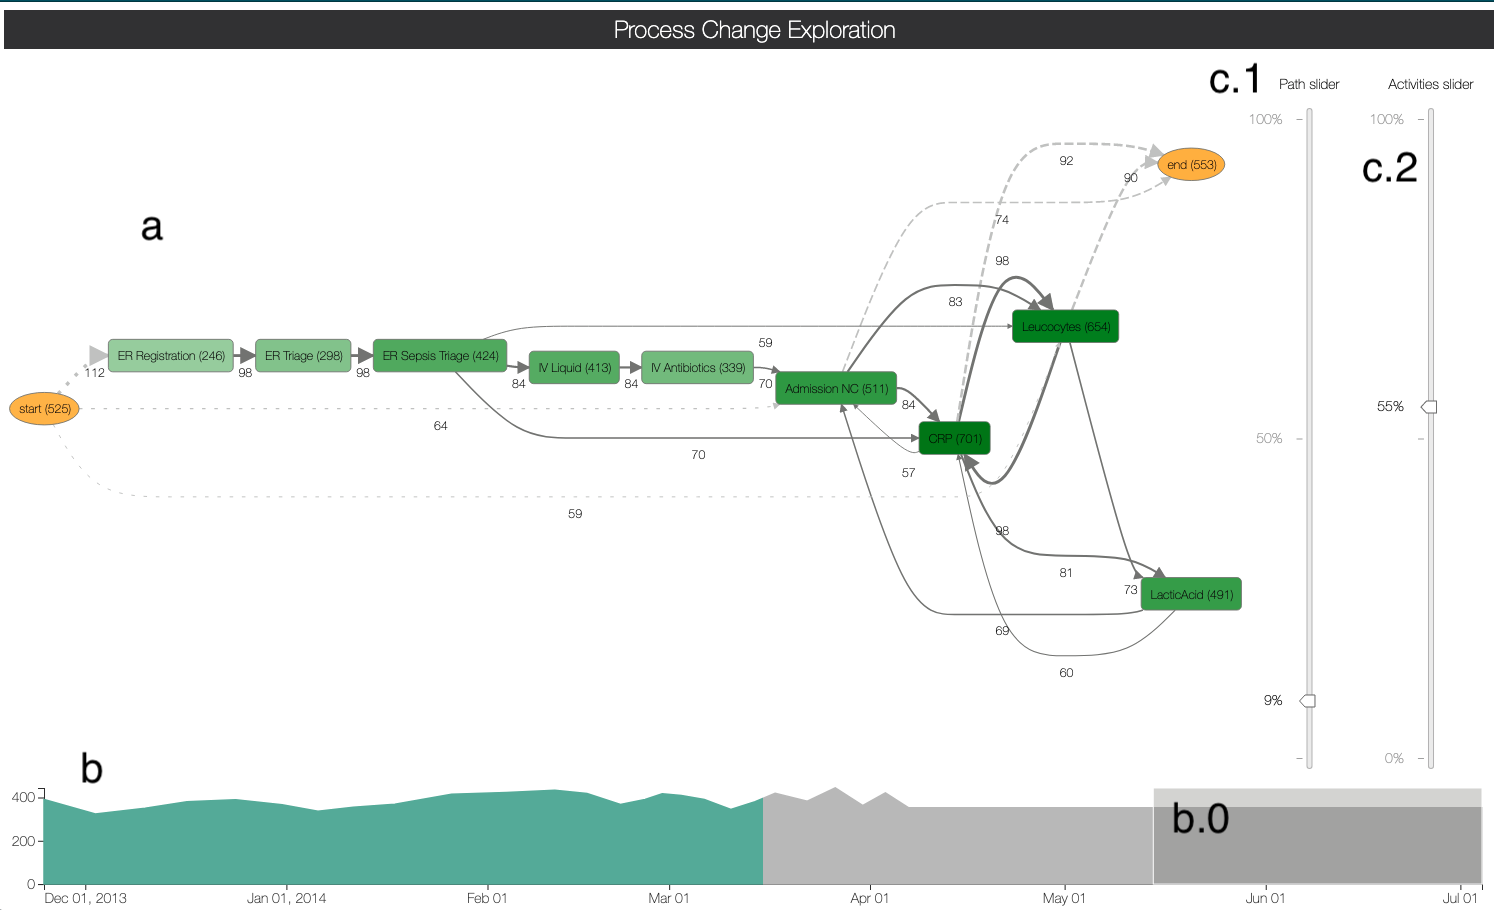
\includegraphics[width=\textwidth]{img/vis/vis-system-one-brush.png}
%	\caption{Process Change Exploration (PCE) system.} 
%	\label{fig:vis-one-brushes}
%\end{figure}

%Process Change Exploration (PCE) system. The interactive system consists of three parts. Part b shows the timeline of the data (green region), and forecasted values (grey region). The user can brush one time range (in this b.0) on this graph to see the filtered for that time range process model. The main view (a) represents the directly follows graph of that region. The c.1 and c.2 are the usual filters on the number of paths and activities to aid simplification the visual representation}

%
%\noindent\textbf{%
%Implementation. 
%} 


%\noindent\textbf{%
%	User interface
%} The Figure~\ref{fig:vis-two-brushes} displays the screenshot of the PCE visualization system. 
%We improve upon the notion of Directly-Follows graph~\cite{leemans2019directly} that is widely used in process mining research and practice. We use the ideas from the version graph~\cite{DBLP:conf/grapp/KriglsteinR12} on how to represent the change between versions of the graph with coloring of the transitions. 

\section{Conclusion}\label{sec:conclusion}
In this paper we investigated the potential of using time series forecasting for process model monitoring.

In future research we will cover more intricate forecasting techniques and compare with machine learning-based models.
Furthermore, we will perform an extensive prediction confidence interval analysis.

\bibliographystyle{splncs03}
\bibliography{lib}

\end{document}
